\chapter{Réactions acido-basiques : dosages et solutions tampons}

\textit{Les réactions acido-basiques sont au cœur de nombreux processus chimiques, biologiques et industriels. Le dosage (ou titrage) acido-basique permet de déterminer la concentration inconnue d'une espèce acide ou basique. Les solutions tampons, quant à elles, jouent un rôle fondamental dans la régulation du pH des milieux biologiques et des réactions chimiques. Ce chapitre développe les aspects théoriques et pratiques de ces concepts essentiels.}

\section{Rappels sur les réactions acido-basiques}

\subsection{Définition d'un acide et d'une base selon Brönsted}

\begin{definition}[Acide et base selon Brönsted]
Un \textbf{acide} est une espèce chimique capable de céder un proton $\ce{H+}$. Une \textbf{base} est une espèce chimique capable de capter un proton $\ce{H+}$.
\end{definition}

\begin{exemple}
\begin{itemize}
    \item Acide chlorhydrique : $\ce{HCl -> H+ + Cl-}$ (acide fort)
    \item Acide éthanoïque : $\ce{CH3COOH <=> H+ + CH3COO-}$ (acide faible)
    \item Ion hydroxyde : $\ce{HO- + H+ -> H2O}$ (base forte)
    \item Ammoniac : $\ce{NH3 + H+ <=> NH4+}$ (base faible)
\end{itemize}
\end{exemple}

\subsection{Couple acide-base et réaction acido-basique}

\begin{definition}[Couple acide-base]
Un \textbf{couple acide-base} est constitué de deux espèces chimiques qui diffèrent par un proton $\ce{H+}$. On le note $\ce{AH/A-}$ où $\ce{AH}$ est l'acide et $\ce{A-}$ la base conjuguée.
\end{definition}

\begin{exemple}
\begin{itemize}
    \item $\ce{CH3COOH/CH3COO-}$ : acide éthanoïque / ion éthanoate
    \item $\ce{NH4+/NH3}$ : ion ammonium / ammoniac
    \item $\ce{H2O/HO-}$ : eau / ion hydroxyde
    \item $\ce{H3O+/H2O}$ : ion oxonium / eau
\end{itemize}
\end{exemple}

\begin{loi}[Réaction acido-basique]
Une \textbf{réaction acido-basique} est le transfert d'un proton $\ce{H+}$ de l'acide d'un couple vers la base d'un autre couple. L'équation générale s'écrit :
\[\ce{AH1 + B2 <=> A1- + BH2+}\]
où $\ce{AH1/A1-}$ et $\ce{BH2+/B2}$ sont les deux couples acide-base mis en jeu.
\end{loi}

\begin{exemple}
Réaction entre l'acide éthanoïque et l'ammoniac :
\[\ce{CH3COOH + NH3 <=> CH3COO- + NH4+}\]
Couples : $\ce{CH3COOH/CH3COO-}$ et $\ce{NH4+/NH3}$.
\end{exemple}

\subsection{Constante d'acidité et force des acides et bases}

\begin{definition}[Constante d'acidité]
Pour un couple acide-base $\ce{AH/A-}$, la \textbf{constante d'acidité} $K_a$ est définie par :
\[K_a = \frac{[\ce{A-}][\ce{H3O+}]}{[\ce{AH}]}\]
On définit également le $\mathrm{p}K_a = -\log K_a$.
\end{definition}

\begin{propriete}[Force des acides et des bases]
\begin{itemize}
    \item Un acide est d'autant plus fort que son $K_a$ est grand (ou son $\mathrm{p}K_a$ petit).
    \item Une base est d'autant plus forte que son $K_a$ est petit (ou son $\mathrm{p}K_a$ grand).
    \item Un acide fort est totalement dissocié dans l'eau : $\ce{AH + H2O -> A- + H3O+}$.
    \item Une base forte est totalement dissociée dans l'eau : $\ce{B + H2O -> BH+ + HO-}$.
\end{itemize}
\end{propriete}

\begin{aretenir}
Pour un acide fort, $K_a \to \infty$ et $\mathrm{p}K_a < 0$. Pour une base forte, $\mathrm{p}K_a > 14$. Les acides et bases faibles ont des $\mathrm{p}K_a$ compris entre 0 et 14.
\end{aretenir}

\subsection{Constante d'équilibre d'une réaction acido-basique}

\begin{loi}[Constante d'équilibre]
Pour une réaction acido-basique $\ce{AH1 + B2 <=> A1- + BH2+}$, la constante d'équilibre $K$ s'exprime en fonction des constantes d'acidité des deux couples :
\[K = \frac{K_{a1}}{K_{a2}} = 10^{\mathrm{p}K_{a2} - \mathrm{p}K_{a1}}\]
où $K_{a1}$ est la constante d'acidité du couple $\ce{AH1/A1-}$ et $K_{a2}$ celle du couple $\ce{BH2+/B2}$.
\end{loi}

\begin{exemple}
Pour la réaction $\ce{CH3COOH + NH3 <=> CH3COO- + NH4+}$ :
\begin{itemize}
    \item $\mathrm{p}K_a(\ce{CH3COOH/CH3COO-}) = 4,8$
    \item $\mathrm{p}K_a(\ce{NH4+/NH3}) = 9,2$
    \item $K = 10^{9,2 - 4,8} = 10^{4,4} \approx 2,5 \times 10^4$
\end{itemize}
La réaction est très favorable dans le sens direct.
\end{exemple}

\section{Dosage (titrage) acido-basique}

\subsection{Principe général du dosage}

\begin{definition}[Dosage acido-basique]
Un \textbf{dosage} (ou titrage) acido-basique est une technique qui consiste à déterminer la concentration inconnue d'une espèce acide ou basique (le \textbf{analyte}) en la faisant réagir avec une solution de concentration connue (le \textbf{titrant} ou réactif titrant).
\end{definition}

\begin{experience}[Montage d'un dosage pH-métrique]
Le montage typique comprend :
\begin{itemize}
    \item Un bécher contenant un volume précis $V_a$ de la solution à doser (acide ou base).
    \item Une burette graduée contenant la solution titrante de concentration $C_b$ connue.
    \item Un pH-mètre avec électrode plongeant dans la solution.
    \item Un agitateur magnétique pour homogénéiser.
\end{itemize}
On ajoute progressivement la solution titrante et on mesure le pH après chaque ajout.
\end{experience}

\subsection{Équivalence d'un dosage}

\begin{definition}[Point d'équivalence]
Le \textbf{point d'équivalence} d'un dosage acido-basique est le point où les réactifs ont été mélangés dans les proportions stœchiométriques de la réaction de dosage. À l'équivalence, les quantités de matière d'acide et de base sont égales.
\end{definition}

\begin{loi}[Relation à l'équivalence]
Pour un dosage d'un acide $\ce{AH}$ par une base $\ce{B}$ (ou l'inverse), la réaction de dosage s'écrit :
\[\ce{AH + B -> A- + BH+}\]
À l'équivalence, on a :
\[n_{\text{acide}} = n_{\text{base}} \quad \text{soit} \quad C_a V_a = C_b V_{b,\text{éq}}\]
où $V_{b,\text{éq}}$ est le volume de solution titrante versé à l'équivalence.
\end{loi}

\begin{exemple}
On dose $V_a = \SI{20,0}{\mL}$ d'une solution d'acide chlorhydrique $\ce{HCl}$ de concentration inconnue $C_a$ par une solution d'hydroxyde de sodium $\ce{NaOH}$ de concentration $C_b = \SI{0,100}{\mol\per\litre}$. L'équivalence est atteinte pour $V_{b,\text{éq}} = \SI{15,0}{\mL}$.
\[C_a = \frac{C_b V_{b,\text{éq}}}{V_a} = \frac{\SI{0,100}{\mol\per\litre} \times \SI{15,0}{\mL}}{\SI{20,0}{\mL}} = \SI{0,0750}{\mol\per\litre}\]
\end{exemple}

\subsection{Suivi pH-métrique et courbe de dosage}

\begin{definition}[Courbe de dosage pH-métrique]
La \textbf{courbe de dosage} est le graphique représentant l'évolution du pH en fonction du volume $V_b$ de solution titrante versé. Elle permet de déterminer le point d'équivalence et d'étudier les propriétés acido-basiques des espèces.
\end{definition}

\subsubsection{Dosage acide fort / base forte}

\begin{experience}[Dosage $\ce{HCl}$ par $\ce{NaOH}$]
La réaction de dosage est :
\[\ce{H3O+ + HO- -> 2 H2O}\]
La constante d'équilibre est $K = \frac{1}{K_e} = 10^{14}$, la réaction est totale.
\end{experience}

\begin{propriete}[Caractéristiques de la courbe]
\begin{itemize}
    \item pH initial : $\mathrm{pH} = -\log C_a$ (pour un acide fort).
    \item Avant l'équivalence : le pH augmente lentement, la solution contient l'acide en excès.
    \item À l'équivalence : $\mathrm{pH} = 7$ (solution neutre).
    \item Après l'équivalence : le pH augmente rapidement, la solution contient la base en excès.
    \item Le saut de pH à l'équivalence est très marqué (plusieurs unités de pH).
\end{itemize}
\end{propriete}

\begin{illus}
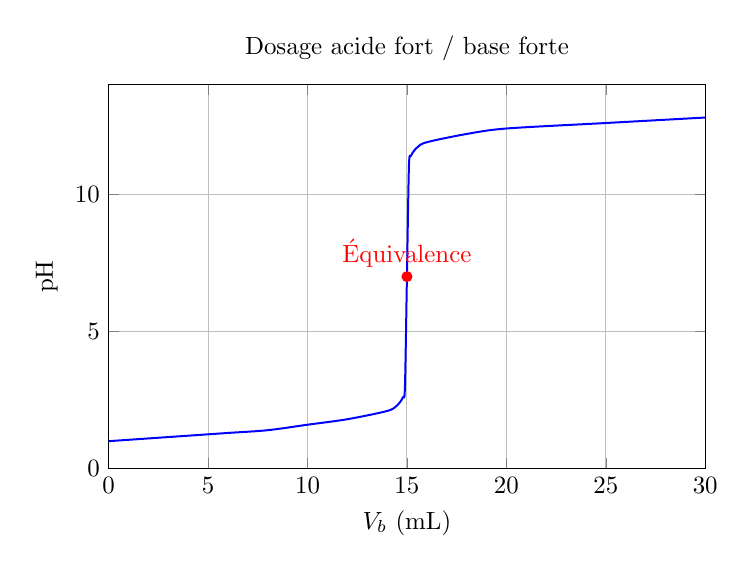
\begin{tikzpicture}[scale=0.9]
\begin{axis}[
    xlabel={$V_b$ (mL)},
    ylabel={pH},
    xmin=0, xmax=30,
    ymin=0, ymax=14,
    grid=both,
    width=10cm,
    height=7cm,
    title={Dosage acide fort / base forte}
]
\addplot[thick, blue, smooth] coordinates {
    (0, 1.0)
    (2, 1.1)
    (4, 1.2)
    (6, 1.3)
    (8, 1.4)
    (10, 1.6)
    (12, 1.8)
    (14, 2.1)
    (14.5, 2.3)
    (14.8, 2.6)
    (14.9, 3.0)
    (15.0, 7.0)
    (15.1, 11.0)
    (15.2, 11.4)
    (15.5, 11.7)
    (16, 11.9)
    (18, 12.2)
    (20, 12.4)
    (25, 12.6)
    (30, 12.8)
};
\addplot[mark=*, only marks, red] coordinates {(15,7)};
\node[red, above] at (axis cs:15,7) {Équivalence};
\end{axis}
\end{tikzpicture}
\fig{Courbe de dosage d'un acide fort par une base forte}
\end{illus}

\subsubsection{Dosage acide faible / base forte}

\begin{experience}[Dosage $\ce{CH3COOH}$ par $\ce{NaOH}$]
La réaction de dosage est :
\[\ce{CH3COOH + HO- -> CH3COO- + H2O}\]
La constante d'équilibre est $K = \frac{K_a}{K_e} = 10^{\mathrm{p}K_e - \mathrm{p}K_a} = 10^{14 - 4,8} = 10^{9,2}$, la réaction est totale.
\end{experience}

\begin{propriete}[Caractéristiques de la courbe]
\begin{itemize}
    \item pH initial : $\mathrm{pH} = \frac{1}{2}(\mathrm{p}K_a - \log C_a)$ (pour un acide faible).
    \item Avant l'équivalence : la solution est une solution tampon (mélange acide faible/base conjuguée).
    \item À la demi-équivalence ($V_b = V_{b,\text{éq}}/2$) : $\mathrm{pH} = \mathrm{p}K_a$.
    \item À l'équivalence : $\mathrm{pH} > 7$ (solution basique car la base conjuguée $\ce{A-}$ est faible).
    \item Après l'équivalence : le pH rejoint la courbe de l'acide fort/base forte.
    \item Le saut de pH à l'équivalence est moins marqué que pour un acide fort.
\end{itemize}
\end{propriete}

\begin{illus}
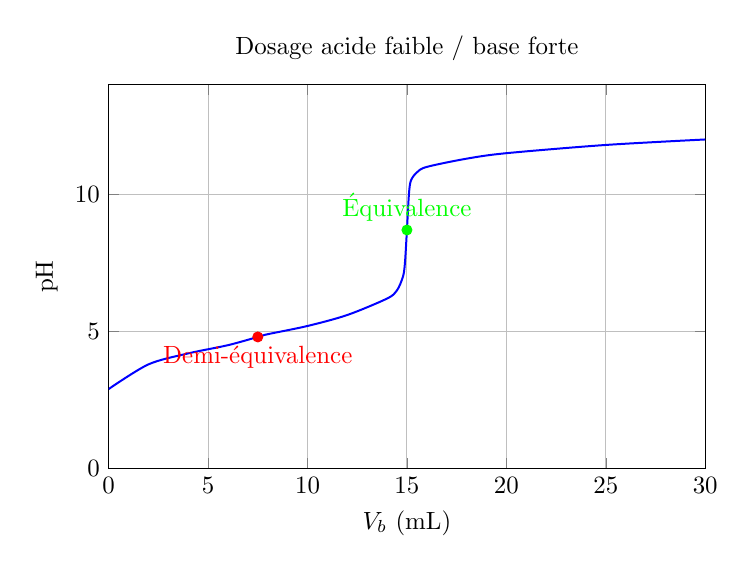
\begin{tikzpicture}[scale=0.9]
\begin{axis}[
    xlabel={$V_b$ (mL)},
    ylabel={pH},
    xmin=0, xmax=30,
    ymin=0, ymax=14,
    grid=both,
    width=10cm,
    height=7cm,
    title={Dosage acide faible / base forte}
]
\addplot[thick, blue, smooth] coordinates {
    (0, 2.9)
    (2, 3.8)
    (4, 4.2)
    (6, 4.5)
    (7.5, 4.8)
    (8, 4.9)
    (10, 5.2)
    (12, 5.6)
    (14, 6.2)
    (14.5, 6.5)
    (14.8, 7.0)
    (14.9, 7.5)
    (15.0, 8.7)
    (15.1, 10.0)
    (15.2, 10.5)
    (15.5, 10.8)
    (16, 11.0)
    (18, 11.3)
    (20, 11.5)
    (25, 11.8)
    (30, 12.0)
};
\addplot[mark=*, only marks, red] coordinates {(7.5,4.8)};
\node[red, below] at (axis cs:7.5,4.8) {Demi-équivalence};
\addplot[mark=*, only marks, green] coordinates {(15,8.7)};
\node[green, above] at (axis cs:15,8.7) {Équivalence};
\end{axis}
\end{tikzpicture}
\fig{Courbe de dosage d'un acide faible par une base forte}
\end{illus}

\subsection{Choix de l'indicateur coloré}

\begin{definition}[Indicateur coloré acido-basique]
Un \textbf{indicateur coloré} est une espèce chimique dont la couleur varie en fonction du pH du milieu. Il se présente sous la forme d'un couple acide-base $\ce{HInd/Ind-}$ dont les deux formes ont des couleurs différentes.
\end{definition}

\begin{propriete}[Zone de virage]
La \textbf{zone de virage} d'un indicateur coloré est la plage de pH dans laquelle la couleur de l'indicateur change. Elle est centrée sur le $\mathrm{p}K_a$ de l'indicateur et s'étend généralement sur $\mathrm{p}K_a \pm 1$.
\end{propriete}

\begin{exemple}[Indicateurs courants]
\begin{itemize}
    \item Hélianthine : zone de virage 3,1--4,4 (rouge $\to$ jaune)
    \item Bleu de bromothymol : zone de virage 6,0--7,6 (jaune $\to$ bleu)
    \item Phénolphtaléine : zone de virage 8,2--10,0 (incolore $\to$ rose)
\end{itemize}
\end{exemple}

\begin{loi}[Choix de l'indicateur]
Pour un dosage acido-basique, l'indicateur coloré doit être choisi de sorte que sa zone de virage contienne le pH à l'équivalence. Ainsi, le changement de couleur sera net et permettra de repérer précisément l'équivalence.
\end{loi}

\begin{exemple}
\begin{itemize}
    \item Dosage acide fort / base forte (pH équivalence = 7) : bleu de bromothymol (6,0--7,6) ou phénolphtaléine (8,2--10,0).
    \item Dosage acide faible / base forte (pH équivalence > 7) : phénolphtaléine (8,2--10,0).
    \item Dosage base faible / acide fort (pH équivalence < 7) : hélianthine (3,1--4,4).
\end{itemize}
\end{exemple}

\section{Solutions tampons}

\subsection{Définition et propriétés}

\begin{definition}[Solution tampon]
Une \textbf{solution tampon} est une solution dont le pH varie très peu lorsqu'on ajoute de petites quantités d'acide ou de base, ou lorsqu'on la dilue modérément.
\end{definition}

\begin{propriete}[Composition d'une solution tampon]
Une solution tampon est généralement constituée d'un mélange d'un acide faible et de sa base conjuguée (ou d'une base faible et de son acide conjugué) en concentrations comparables.
\end{propriete}

\begin{exemple}
\begin{itemize}
    \item Tampon éthanoïque : $\ce{CH3COOH/CH3COO-}$ (mélange d'acide éthanoïque et d'éthanoate de sodium)
    \item Tampon ammoniacal : $\ce{NH4+/NH3}$ (mélange de chlorure d'ammonium et d'ammoniac)
    \item Tampon phosphate : $\ce{H2PO4-/HPO4^2-}$
\end{itemize}
\end{exemple}

\subsection{pH d'une solution tampon : relation d'Henderson-Hasselbalch}

\begin{loi}[Relation d'Henderson-Hasselbalch]
Pour une solution tampon constituée d'un acide faible $\ce{AH}$ et de sa base conjuguée $\ce{A-}$, le pH est donné par :
\[\mathrm{pH} = \mathrm{p}K_a + \log\frac{[\ce{A-}]}{[\ce{AH}]}\]
Cette relation est valable lorsque les concentrations sont suffisamment élevées (généralement $> 10^{-3}$ mol/L).
\end{loi}

\begin{propriete}[Propriété fondamentale]
Lorsque $[\ce{A-}] = [\ce{AH}]$, on a $\mathrm{pH} = \mathrm{p}K_a$. Le pouvoir tampon est maximal dans ces conditions.
\end{propriete}

\begin{exemple}
On prépare une solution tampon en mélangeant $V_a = \SI{50,0}{\mL}$ d'acide éthanoïque $\SI{0,10}{\mol\per\litre}$ et $V_b = \SI{50,0}{\mL}$ d'éthanoate de sodium $\SI{0,10}{\mol\per\litre}$. Le $\mathrm{p}K_a$ de l'acide éthanoïque est 4,8.
\[[\ce{CH3COOH}] = [\ce{CH3COO-}] = \frac{\SI{0,10}{\mol\per\litre} \times \SI{50,0}{\mL}}{\SI{100,0}{\mL}} = \SI{0,050}{\mol\per\litre}\]
\[\mathrm{pH} = 4,8 + \log\frac{0,050}{0,050} = 4,8\]
\end{exemple}

\subsection{Pouvoir tampon}

\begin{definition}[Pouvoir tampon]
Le \textbf{pouvoir tampon} (ou capacité tampon) $\beta$ d'une solution est la quantité d'acide ou de base forte qu'il faut ajouter pour faire varier le pH d'une unité :
\[\beta = \frac{|\Delta n|}{\Delta\mathrm{pH}}\]
où $\Delta n$ est la quantité de matière d'acide ou de base ajoutée et $\Delta\mathrm{pH}$ la variation de pH correspondante.
\end{definition}

\begin{propriete}[Facteurs influençant le pouvoir tampon]
\begin{itemize}
    \item Le pouvoir tampon est maximal lorsque $\mathrm{pH} = \mathrm{p}K_a$ (soit $[\ce{A-}] = [\ce{AH}]$).
    \item Le pouvoir tampon augmente avec les concentrations de l'acide et de sa base conjuguée.
    \item Une solution tampon est efficace dans une zone de pH comprise entre $\mathrm{p}K_a - 1$ et $\mathrm{p}K_a + 1$.
\end{itemize}
\end{propriete}

\begin{exemple}
On considère une solution tampon de volume $V = \SI{100}{\mL}$ contenant $\ce{CH3COOH}$ et $\ce{CH3COO-}$ à $\SI{0,10}{\mol\per\litre}$ chacun. On ajoute $\SI{1,0}{\mL}$ de $\ce{HCl}$ $\SI{1,0}{\mol\per\litre}$.
\begin{itemize}
    \item Quantité de $\ce{H+}$ ajoutée : $n = \SI{1,0e-3}{\mol}$
    \item La réaction $\ce{CH3COO- + H+ -> CH3COOH}$ consomme $\ce{CH3COO-}$ et produit $\ce{CH3COOH}$.
    \item Nouvelles concentrations : $[\ce{CH3COO-}] = \frac{0,010 - 0,001}{0,101} \approx \SI{0,089}{\mol\per\litre}$, $[\ce{CH3COOH}] = \frac{0,010 + 0,001}{0,101} \approx \SI{0,109}{\mol\per\litre}$
    \item Nouveau pH : $\mathrm{pH} = 4,8 + \log\frac{0,089}{0,109} \approx 4,8 - 0,09 = 4,71$
    \item Variation de pH : $\Delta\mathrm{pH} = 4,71 - 4,80 = -0,09$ (très faible)
\end{itemize}
Sans tampon, l'ajout de $\ce{H+}$ dans $\SI{100}{\mL}$ d'eau pure donnerait $\mathrm{pH} \approx 2$, soit une variation de 5 unités !
\end{exemple}

\subsection{Préparation d'une solution tampon}

\begin{experience}[Préparation d'une solution tampon]
Plusieurs méthodes permettent de préparer une solution tampon :
\begin{enumerate}
    \item \textbf{Mélange direct} : dissoudre l'acide faible et sa base conjuguée (sous forme de sel) dans l'eau.
    \item \textbf{Neutralisation partielle} : faire réagir un acide faible avec une base forte (ou l'inverse) en proportions telles qu'il reste de l'acide et de la base conjuguée.
    \item \textbf{Utilisation d'un sel d'acide faible} : dissoudre un sel d'acide faible (ex : $\ce{NaHCO3}$) et ajuster le pH avec un acide ou une base forte.
\end{enumerate}
\end{experience}

\begin{exemple}
Préparation de $\SI{500}{\mL}$ d'une solution tampon de pH = 5,2 à partir d'acide éthanoïque ($\mathrm{p}K_a = 4,8$) et d'éthanoate de sodium.
\[\mathrm{pH} = \mathrm{p}K_a + \log\frac{[\ce{CH3COO-}]}{[\ce{CH3COOH}]} \Rightarrow 5,2 = 4,8 + \log\frac{[\ce{CH3COO-}]}{[\ce{CH3COOH}]}\]
\[\log\frac{[\ce{CH3COO-}]}{[\ce{CH3COOH}]} = 0,4 \Rightarrow \frac{[\ce{CH3COO-}]}{[\ce{CH3COOH}]} = 10^{0,4} \approx 2,5\]
On peut choisir $[\ce{CH3COOH}] = \SI{0,10}{\mol\per\litre}$ et $[\ce{CH3COO-}] = \SI{0,25}{\mol\per\litre}$.
Pour $\SI{500}{\mL}$ :
\begin{itemize}
    \item $n_{\ce{CH3COOH}} = \SI{0,10}{\mol\per\litre} \times \SI{0,500}{\L} = \SI{0,050}{\mol}$
    \item $n_{\ce{CH3COONa}} = \SI{0,25}{\mol\per\litre} \times \SI{0,500}{\L} = \SI{0,125}{\mol}$
\end{itemize}
\end{exemple}

\begin{aretenir}
Les solutions tampons sont essentielles en biologie (sang, $\mathrm{pH} \approx 7,4$), en chimie analytique et dans l'industrie. Le sang humain est tamponné par le système $\ce{H2CO3/HCO3-}$ ($\mathrm{p}K_a = 6,1$) et le système $\ce{H2PO4-/HPO4^2-}$ ($\mathrm{p}K_a = 7,2$).
\end{aretenir}

\section{L'essentiel à retenir}

\begin{synthese}
\subsection*{Réactions acido-basiques}
\begin{itemize}
    \item Un acide cède un proton $\ce{H+}$, une base capte un proton.
    \item Couple acide-base : $\ce{AH/A-}$.
    \item Constante d'acidité : $K_a = \dfrac{[\ce{A-}][\ce{H3O+}]}{[\ce{AH}]}$, $\mathrm{p}K_a = -\log K_a$.
    \item Constante d'équilibre d'une réaction : $K = \dfrac{K_{a1}}{K_{a2}} = 10^{\mathrm{p}K_{a2} - \mathrm{p}K_{a1}}$.
\end{itemize}

\subsection*{Dosage acido-basique}
\begin{itemize}
    \item Équivalence : $C_a V_a = C_b V_{b,\text{éq}}$.
    \item Dosage acide fort / base forte : $\mathrm{pH}_{\text{éq}} = 7$, saut de pH marqué.
    \item Dosage acide faible / base forte : $\mathrm{pH}_{\text{éq}} > 7$, $\mathrm{pH}_{\text{demi-éq}} = \mathrm{p}K_a$.
    \item Choix de l'indicateur : zone de virage doit contenir le pH à l'équivalence.
\end{itemize}

\subsection*{Solutions tampons}
\begin{itemize}
    \item Mélange acide faible / base conjuguée (ou base faible / acide conjugué).
    \item Relation d'Henderson-Hasselbalch : $\mathrm{pH} = \mathrm{p}K_a + \log\dfrac{[\ce{A-}]}{[\ce{AH}]}$.
    \item Pouvoir tampon maximal quand $[\ce{A-}] = [\ce{AH}]$ (soit $\mathrm{pH} = \mathrm{p}K_a$).
    \item Zone d'efficacité : $\mathrm{p}K_a \pm 1$.
\end{itemize}

\subsection*{Pièges à éviter}
\begin{itemize}
    \item Ne pas confondre $\mathrm{p}K_a$ et $\mathrm{pH}$ : $\mathrm{p}K_a$ est une constante, $\mathrm{pH}$ varie.
    \item Pour un acide fort, $\mathrm{pH} = -\log C$ ; pour un acide faible, $\mathrm{pH} = \frac{1}{2}(\mathrm{p}K_a - \log C)$.
    \item À l'équivalence d'un dosage acide faible / base forte, la solution est basique (hydrolyse de $\ce{A-}$).
    \item Le pouvoir tampon n'est pas infini : il est limité par les concentrations.
\end{itemize}
\end{synthese}

\section{Méthodes \& savoir-faire}

\methode{Déterminer la constante d'équilibre d'une réaction acido-basique}
Pour déterminer la constante d'équilibre $K$ d'une réaction entre un acide $\ce{AH1}$ et une base $\ce{B2}$ :
\begin{enumerate}
    \item Identifier les deux couples acide-base : $\ce{AH1/A1-}$ et $\ce{BH2+/B2}$.
    \item Relever les $\mathrm{p}K_a$ des deux couples.
    \item Appliquer la formule : $K = 10^{\mathrm{p}K_{a2} - \mathrm{p}K_{a1}}$.
    \item Interpréter : si $K > 10^4$, la réaction est totale ; si $K < 10^{-4}$, elle est négligeable.
\end{enumerate}

\begin{exemple}
Calculer $K$ pour la réaction $\ce{NH4+ + HO- <=> NH3 + H2O}$.
Données : $\mathrm{p}K_a(\ce{NH4+/NH3}) = 9,2$, $\mathrm{p}K_a(\ce{H2O/HO-}) = 14$.
\[K = 10^{14 - 9,2} = 10^{4,8} \approx 6,3 \times 10^4\]
La réaction est totale.
\end{exemple}

\methode{Calculer le pH d'une solution d'acide ou de base}
\begin{enumerate}
    \item Identifier si l'espèce est forte ou faible.
    \item Si acide fort : $\mathrm{pH} = -\log C$.
    \item Si base forte : $\mathrm{pH} = 14 + \log C$.
    \item Si acide faible : $\mathrm{pH} = \frac{1}{2}(\mathrm{p}K_a - \log C)$ (valable si $C \gg K_a$).
    \item Si base faible : $\mathrm{pH} = 7 + \frac{1}{2}(\mathrm{p}K_a + \log C)$.
\end{enumerate}

\begin{exemple}
Calculer le pH d'une solution d'acide éthanoïque $\SI{0,050}{\mol\per\litre}$ ($\mathrm{p}K_a = 4,8$).
\[\mathrm{pH} = \frac{1}{2}(4,8 - \log 0,050) = \frac{1}{2}(4,8 + 1,3) = \frac{1}{2} \times 6,1 = 3,05\]
\end{exemple}

\methode{Déterminer la concentration inconnue par dosage}
\begin{enumerate}
    \item Réaliser le dosage et repérer le volume à l'équivalence $V_{b,\text{éq}}$.
    \item Écrire l'équation de la réaction de dosage.
    \item Appliquer la relation $C_a V_a = C_b V_{b,\text{éq}}$ (pour un dosage acide-base).
    \item Isoler la concentration inconnue : $C_a = \dfrac{C_b V_{b,\text{éq}}}{V_a}$.
    \item Vérifier la cohérence du résultat (ordre de grandeur, unités).
\end{enumerate}

\begin{exemple}
On dose $\SI{10,0}{\mL}$ d'une solution d'acide chlorhydrique par $\ce{NaOH}$ $\SI{0,200}{\mol\per\litre}$. L'équivalence est à $V_b = \SI{12,5}{\mL}$.
\[C_a = \frac{\SI{0,200}{\mol\per\litre} \times \SI{12,5}{\mL}}{\SI{10,0}{\mL}} = \SI{0,250}{\mol\per\litre}\]
\end{exemple}

\methode{Exploiter une courbe de dosage pour déterminer le $\mathrm{p}K_a$}
Pour un dosage acide faible / base forte :
\begin{enumerate}
    \item Repérer le point d'équivalence (saut de pH).
    \item Déterminer le volume à la demi-équivalence : $V_{b,1/2} = V_{b,\text{éq}}/2$.
    \item Lire le pH correspondant sur la courbe : $\mathrm{pH}_{1/2} = \mathrm{p}K_a$.
\end{enumerate}

\begin{exemple}
Sur la courbe de dosage de l'acide éthanoïque par $\ce{NaOH}$, l'équivalence est à $V_b = \SI{20,0}{\mL}$. À $V_b = \SI{10,0}{\mL}$, le pH est 4,8. Donc $\mathrm{p}K_a(\ce{CH3COOH}) = 4,8$.
\end{exemple}

\methode{Choisir un indicateur coloré adapté}
\begin{enumerate}
    \item Déterminer le pH à l'équivalence du dosage.
    \item Consulter la liste des indicateurs avec leurs zones de virage.
    \item Choisir un indicateur dont la zone de virage contient le pH à l'équivalence.
    \item Vérifier que le changement de couleur est net et visible.
\end{enumerate}

\begin{exemple}
Pour un dosage acide faible / base forte avec $\mathrm{pH}_{\text{éq}} = 8,7$, on choisit la phénolphtaléine (zone 8,2--10,0). L'hélianthine (3,1--4,4) ne convient pas.
\end{exemple}

\methode{Calculer le pH d'une solution tampon}
\begin{enumerate}
    \item Identifier l'acide faible et sa base conjuguée.
    \item Déterminer les concentrations $[\ce{AH}]$ et $[\ce{A-}]$ après mélange.
    \item Appliquer la relation d'Henderson-Hasselbalch : $\mathrm{pH} = \mathrm{p}K_a + \log\frac{[\ce{A-}]}{[\ce{AH}]}$.
    \item Vérifier que les concentrations sont suffisantes ($> 10^{-3}$ mol/L).
\end{enumerate}

\begin{exemple}
On mélange $\SI{100}{\mL}$ de $\ce{CH3COOH}$ $\SI{0,20}{\mol\per\litre}$ et $\SI{100}{\mL}$ de $\ce{CH3COONa}$ $\SI{0,30}{\mol\per\litre}$. $\mathrm{p}K_a = 4,8$.
\begin{itemize}
    \item $[\ce{CH3COOH}] = \frac{0,20 \times 0,100}{0,200} = \SI{0,10}{\mol\per\litre}$
    \item $[\ce{CH3COO-}] = \frac{0,30 \times 0,100}{0,200} = \SI{0,15}{\mol\per\litre}$
    \item $\mathrm{pH} = 4,8 + \log\frac{0,15}{0,10} = 4,8 + \log 1,5 = 4,8 + 0,18 = 4,98$
\end{itemize}
\end{exemple}

\methode{Préparer une solution tampon de pH donné}
\begin{enumerate}
    \item Choisir un couple acide-base dont le $\mathrm{p}K_a$ est proche du pH désiré (à $\pm 1$ unité).
    \item Utiliser la relation d'Henderson-Hasselbalch pour déterminer le rapport $\frac{[\ce{A-}]}{[\ce{AH}]}$.
    \item Choisir une concentration totale convenable (généralement entre 0,01 et 0,1 mol/L).
    \item Calculer les masses ou volumes nécessaires pour préparer la solution.
\end{enumerate}

\begin{exemple}
Préparer $\SI{250}{\mL}$ d'une solution tampon de pH = 7,4 avec le système $\ce{H2PO4-/HPO4^2-}$ ($\mathrm{p}K_a = 7,2$).
\[7,4 = 7,2 + \log\frac{[\ce{HPO4^2-}]}{[\ce{H2PO4-}]} \Rightarrow \frac{[\ce{HPO4^2-}]}{[\ce{H2PO4-}]} = 10^{0,2} \approx 1,58\]
On choisit $[\ce{H2PO4-}] = \SI{0,050}{\mol\per\litre}$ et $[\ce{HPO4^2-}] = \SI{0,079}{\mol\per\litre}$.
Masses pour $\SI{250}{\mL}$ :
\begin{itemize}
    \item $m_{\ce{KH2PO4}} = \SI{0,050}{\mol\per\litre} \times \SI{0,250}{\L} \times \SI{136,1}{\gram\per\mol} = \SI{1,70}{\gram}$
    \item $m_{\ce{K2HPO4}} = \SI{0,079}{\mol\per\litre} \times \SI{0,250}{\L} \times \SI{174,2}{\gram\per\mol} = \SI{3,44}{\gram}$
\end{itemize}
\end{exemple}

\methode{Calculer la variation de pH après ajout d'acide ou de base à une solution tampon}
\begin{enumerate}
    \item Écrire l'équation de la réaction entre l'espèce ajoutée et le composant du tampon.
    \item Calculer les nouvelles quantités de matière de l'acide et de la base conjuguée.
    \item Calculer les nouvelles concentrations en tenant compte de la dilution.
    \item Appliquer la relation d'Henderson-Hasselbalch pour trouver le nouveau pH.
    \item Comparer avec la variation qu'aurait subie l'eau pure.
\end{enumerate}

\begin{exemple}
À $\SI{100}{\mL}$ d'une solution tampon $\ce{CH3COOH/CH3COO-}$ $\SI{0,10}{\mol\per\litre}$ (pH = 4,8), on ajoute $\SI{5,0}{\mL}$ de $\ce{HCl}$ $\SI{0,10}{\mol\per\litre}$.
\begin{itemize}
    \item $n_{\ce{H+}}$ ajouté = $\SI{0,10}{\mol\per\litre} \times \SI{0,0050}{\L} = \SI{5,0e-4}{\mol}$
    \item $n_{\ce{CH3COO-}}$ initial = $\SI{0,10}{\mol\per\litre} \times \SI{0,100}{\L} = \SI{1,0e-2}{\mol}$
    \item $n_{\ce{CH3COOH}}$ initial = $\SI{1,0e-2}{\mol}$
    \item Après réaction : $n_{\ce{CH3COO-}} = 1,0\times10^{-2} - 5,0\times10^{-4} = \SI{9,5e-3}{\mol}$
    \item $n_{\ce{CH3COOH}} = 1,0\times10^{-2} + 5,0\times10^{-4} = \SI{1,05e-2}{\mol}$
    \item Volume total = $\SI{0,105}{\L}$
    \item $[\ce{CH3COO-}] = \frac{9,5\times10^{-3}}{0,105} = \SI{0,0905}{\mol\per\litre}$
    \item $[\ce{CH3COOH}] = \frac{1,05\times10^{-2}}{0,105} = \SI{0,100}{\mol\per\litre}$
    \item $\mathrm{pH} = 4,8 + \log\frac{0,0905}{0,100} = 4,8 - 0,043 = 4,76$
    \item Variation : $\Delta\mathrm{pH} = -0,04$ (très faible)
\end{itemize}
\end{exemple}

\methode{Interpréter le pouvoir tampon d'une solution}
\begin{enumerate}
    \item Calculer le rapport $[\ce{A-}]/[\ce{AH}]$ : plus il est proche de 1, plus le pouvoir tampon est élevé.
    \item Vérifier que le pH est dans la zone $\mathrm{p}K_a \pm 1$.
    \item Évaluer les concentrations : plus elles sont élevées, plus le pouvoir tampon est grand.
    \item Pour comparer deux solutions tampons, calculer $\beta = \frac{|\Delta n|}{\Delta\mathrm{pH}}$ pour un même ajout.
\end{enumerate}

\begin{exemple}
Deux solutions tampons de même volume ($\SI{100}{\mL}$) :
\begin{itemize}
    \item Tampon A : $[\ce{AH}] = [\ce{A-}] = \SI{0,10}{\mol\per\litre}$
    \item Tampon B : $[\ce{AH}] = [\ce{A-}] = \SI{0,010}{\mol\per\litre}$
\end{itemize}
Pour un ajout de $\SI{1,0}{\mL}$ de $\ce{HCl}$ $\SI{0,10}{\mol\per\litre}$ :
\begin{itemize}
    \item Tampon A : $\Delta\mathrm{pH} \approx -0,04$ (fort pouvoir tampon)
    \item Tampon B : $\Delta\mathrm{pH} \approx -0,4$ (pouvoir tampon plus faible)
\end{itemize}
Le tampon A a un meilleur pouvoir tampon car ses concentrations sont plus élevées.
\end{exemple}